%!TEX TS-program = pdflatex
%!TEX root = thesis.tex
%\documentclass[10pt,a4paper,onecolumn,twoside,openright]{book}
\let\accentvec\vec
\documentclass[10pt,a4paper,onecolumn,twoside,openright,titlepage]{svmono}
\let\spvec\vec
\let\vec\accentvec
% added by me
\usepackage{siunitx}

\usepackage{amssymb}
\usepackage[english]{varioref}		% Vario REF \vref
\usepackage{hyperref}			% Clickable links
\usepackage{url}
%\usepackage{graphics}
\usepackage{graphicx}							% Graphic support for eps
\usepackage[utf8]{inputenc}		% Input Encoding auf Windows einstellen
\usepackage[T1]{fontenc}					% Umlaute unterstützen
%\usepackage{ams}
\usepackage{textcomp}							% TC fonts
\usepackage{color}
%\usepackage{alltt}								% includes verbatim from text files
\usepackage{lmodern}							% Schriftanpassungen
\usepackage{multicol}							% Mehrere Spalten im Text verwenden
%\usepackage[bottom]{footmisc}			% Fußzeilen
\usepackage{pifont} 							% for fancy bullets
\usepackage{setspace}							% Zeilenabstand
\usepackage{fancyhdr}							% Kopfzeilen
\usepackage{makeidx}							% Index
\usepackage[english]{babel}				%	nationale Datumsformate, etc.
\usepackage{nomencl}							% Erstellt Abkürzungsverzeichnisse
%\usepackage[style=long,border=none,header=plain,cols=2,number=none,hypertoc=true,acronym=false,global=true]{glossary}   %
\usepackage{tabularx}							% Tabellen mit Type X haben automatische minipage mit Zeilenumbruch
\usepackage{multirow}
\usepackage{rotating}             % Rotieren von float elementen
\usepackage{booktabs}							% Tabellen verschönern mit toprule/bottomrule
\usepackage{colortbl}							% farbige Tabellen
\usepackage[numbers, sort]{natbib}								% Naturwissenschaftliches Zitieren
%\usepackage[small, normal, bf, up]{caption2} % Paket für schönere Bildunterschriften
%\usepackage[nottoc]{tocbibind}		% Literaturverzeichnis in Inhaltsverzeichnis aufnehmen
\usepackage{listings} % Programm-Listing
\lstset{language=C}
\usepackage{float}
\usepackage{amsmath}
\usepackage{parskip}
%\usepackage[toc,nonumberlist]{glossaries}
\usepackage[acronym,nomain]{glossaries}
\usepackage[toc]{appendix}
\usepackage{algorithm}
\usepackage{chngcntr}
\usepackage{algpseudocode}
%\usepackage{algorithmic}
\usepackage{xspace} % solves problem with missing space after \newcommand
\usepackage[capitalise]{cleveref} % use for \cref command

% http://homepage.ruhr-uni-bochum.de/Georg.Verweyen/pakete.html
\usepackage{ellipsis}
\usepackage{microtype}

% architecture figure
\usepackage{tikz}
\usetikzlibrary{shapes,arrows}

%\counterwithout{footnote}{chapter}

\fancypagestyle{plain}{										% Redefining the plain style
	\fancyhf{}
	\renewcommand{\headrulewidth}{0pt}
	\renewcommand{\footrulewidth}{0pt}
}

\crefname{chapter}{Chapter}{Chapters}
\crefname{section}{Section}{Sections}
\Crefname{chapter}{Chapter}{Chapters}
\Crefname{section}{Section}{Sections}
\crefname{equation}{}{}


%Kopf- und Fußzeile
\pagestyle{fancy}																		% {fancyhdr}: besetzt Kopf- und Fusszeilen mit definiertem Inhalt
\fancyhf{}																					% clear all header and footer fields
																										% im Stil slanted-shape = geneigt; nouppercase = klein geschrieben
\fancyhead[LE,RO]{\bfseries \thepage}								% LE=left-even + RO=right-odd: \thepage=Seitenzahl
\fancyhead[LO]{\bfseries \nouppercase{\rightmark}}		% LO=left-odd: \rightmark=lower-level sectioning information
\fancyhead[RE]{\bfseries \nouppercase{\leftmark}}		% RE=right-even: \leftmark=higher-level sectioning information
\renewcommand{\headrulewidth}{0.5pt}								% Linie zum Abtrennen der Kopfzeile mit entsprechender Breite
\renewcommand{\footrulewidth}{0pt}									% Linie zum Abtrennen der Fusszeile mit entsprechender Breite (0=keine Linie)
%\setlength\headheight{13.6pt}
\headheight 13.6pt																	% wegen Schriftgröße 11pt muss die Höhe der Kopfzeile vergrößert werden

%\setacronymnamefmt{\gloshort}  % setzt den ersten Wert im Abkürzungsverzeichnis auf die Abkürzung selbst
%\setacronymdescfmt{\glolong: \glodesc}
%\makeacronym
%\newglossarystyle{modsuper}{
%  \glossarystyle{super}
%  \renewcommand{\glsgroupskip}{}
%}
\makeindex
%\makeglossary
%\makeglossaries

% Punkte zw. Abkürzung und Erklärung für Abkürzungsverzeichnis
\setlength{\nomlabelwidth}{.20\hsize}
\renewcommand{\nomlabel}[1]{#1 \dotfill}
%\makenomenclature


%\bibliographystyle{unsrtnat}
%\bibliographystyle{unsrt}
\bibliographystyle{acm}
%\bibliographystyle{ieeetr}
\newcommand*{\Mail}[1]{\href{mailto:#1}{\protect\url{#1}}}
\newcommand*{\MailTitle}[2]{\href{mailto:#1@#2}{\protect\url{#1}}}
\newcommand{\keywords}[1]{\par\addvspace\baselineskip\noindent\keywordname\enspace\ignorespaces#1}
\newcommand{\biburl}[2]{\url{#1} (last visited #2)}
\newcommand{\itembf}[1]{\item \textbf{#1}}
\newcommand{\blankpage}{\clearpage{\pagestyle{empty}\cleardoublepage}}

%\def\thechapter{\Alph{chapter}}
%\def\thesection{\arabic{section}}

\onehalfspacing % {setspace}: setzt den Zeilenabstand auf 1,5
% Ränder definieren
\oddsidemargin 1in
\evensidemargin 0.5in

\renewcommand{\arraystretch}{1.5}
\renewcommand{\tabcolsep}{6pt}
\selectlanguage{english}

\definecolor{grey}{rgb}{0.85,0.85,0.85}
\definecolor{hpi_orange}{rgb}{0.88, 0.43, 0.20}
\definecolor{hpi}{rgb}{0.537,0.063,0.165}

\newcommand{\TITLE}{Data-Driven Order and Pricing Optimization on Online Marketplaces}
%remove german title?
\newcommand{\TITLEGERMAN}{Datengetriebene Bestell- und Preisoptimierung auf einem Online-Marktplatz}
% "auf einem Online-Marktplatz" klingt doof, aber "auf Online-Marktplätzen" wäre falsch
\newcommand{\AUTHOR}{Carsten Walther}
\newcommand{\EMAIL}{carsten.walther@student.hpi.de}
\newcommand{\pricewars}{Price Wars\xspace}

\lstset{breaklines=true,
    numbersep=5pt,
 	stepnumber=1,
	numbers=left,
	captionpos=b,
	float=htbp,
    basicstyle=\ttfamily\fontsize{9}{12}\selectfont
}
\lstset{frame=tb, aboveskip=0.5cm, belowskip=0.5cm}

\newcommand{\todo}[1]{
  \textbf{\textcolor{hpi}{TODO #1}}
}

\newacronym{NVRAM}{NVRAM}{non-volatile random-access memory}


\begin{document}
	%!TEX root = thesis.tex
\begin{titlepage}

\thispagestyle{empty}
\begin{center}
	\LARGE
	Master's Thesis\\
	\vspace{0.4cm}
	\Huge
    \TITLE{}\\
	\vspace{0.4cm}
	%\large
    %\TITLEGERMAN{}\\
	\vspace{0.5cm}
	\LARGE
	\textbf{\AUTHOR}\\
	\normalsize
  \Mail{\EMAIL}\\
	\vspace{0.4cm}
	\small
	Hasso Plattner Institute for IT Systems Engineering\\
	Enterprise Platform and Integration Concepts Chair\\
	\vspace{0.3cm}
	\raisebox{0.5\height}{
\includegraphics[width=3cm]{figures/hpi_logo.pdf}}
	\hspace{1cm}
	
\includegraphics[width=3cm]{figures/Universitaet_Potsdam_logo}\\
	\vspace{0.1cm}
	August-Bebel-Str. 88\\
	14482 Potsdam, Germany\\
	\url{https://hpi.de/plattner}\\
%	\vspace{1.5cm}
\end{center}
%\begin{minipage}[b]{\textwidth}
\vspace{0.7cm}
Supervisors:
\vspace{0.3cm}\\
%\begin{minipage}[b]{0.45\linewidth}
Prof. Dr. Hasso Plattner\\
Dr. Matthias Uflacker\\
Dr. Rainer Schlosser\\
Martin Boissier\\
\vspace{0.3cm}\\
Hasso Plattner Institute\\
Potsdam, Germany
%\end{minipage}
\vspace{0.4cm}\\
\today
%\end{minipage}
\end{titlepage}

	\pagestyle{empty}
	\cleardoublepage

	\pagestyle{fancy}
	\pagenumbering{roman}
	%!TEX root = ../thesis.tex
\chapter*{Abstract}
%situation
Online marketplaces become increasingly competitive.
Merchants dynamically adjust offer prices to get an advantage over the competition.
They have to estimate demand to prevent understocking and overstocking.
%problem
Finding optimal pricing and ordering strategies is challenging because demand is uncertain, sales are affected by competitors' prices, and pricing and ordering decisions are mutually dependent.
Merchants' pricing and ordering decisions determine their profitability and economic viability.
%solution
We derived an optimization approach that utilizes dynamic programming to create profit maximizing pricing and ordering policies.
Demand is estimated based on historical market data using demand learning with linear regression.
We implemented the optimization approach in a merchant and tested it on the \pricewars platform in different scenarios against other merchants.
%result:
Our merchant outperforms rule-based merchants if enough trainings data is available.

%platform motivation
Testing merchant strategies in production is time-consuming and potentially costly.
The \pricewars platform is an open-source simulation framework that gives researcher and practitioners the opportunity to test and evaluate merchant strategies in competitive marketplace environments.
%what we done
We extended the platform by inventory holding costs, fixed order costs, and order delivery delay to make ordering decisions more crucial for profit maximization.
%why we done
This extensions allows testing merchant strategies under more realistic conditions.
	\clearpage
	\glsresetall
	\setcounter{page}{0}
	\setcounter{tocdepth}{4}
	\tableofcontents
	\glsresetall
	\cleardoublepage
	\phantomsection \label{listoffig}
%	\addcontentsline{toc}{section}{List of Figures}
	\listoffigures
	\glsresetall
	
	%\phantomsection \label{listoflst}
	%\lstlistoflistings
	%\glsresetall
	%\newpage
	
%	\phantomsection \label{listoftab}
%	\addcontentsline{toc}{section}{List of Tables}
%	\listoftables
%	\newpage
	\glsresetall
	\pagenumbering {arabic}
	\setcounter{page}{0}
	%!TEX root = ../thesis.tex

\chapter{Introduction}
%Why dynamic pricing?
Price updates on today's online markets increase in number and happen in shorter intervals.
Merchants want an advantage by adjusting their prices to competitors' prices.
The frequent updating of prices is called dynamic pricing and is used by merchants to increase their profit compared to traditional pricing strategies.
Human agents lack the fast response times and endurance to compete with software agents.
Additionally, these programs are able to analyze huge amounts of historical market data and can estimate customer buying behavior from it.
%Online marketplaces are ideal environments to apply dynamic pricing strategies because there is almost no cost for price changes.
%human irrational decisions

%Why inventory control?
Another important task of a merchant is keeping track of the inventory.
If the inventory level is to low, the merchant might miss potential sales due to a stock-out.
But storing to many items causes preventable extra costs.
This is the inventory control problem and it is about when to order how many new products.
It is crucial to accurately predict future demand for good order decisions.
%todo put following sentence somewhere after costs are introduced
%The merchant wants to find a good balance between few big orders, which minimizes fixed order costs, and many small orders, which minimizes holding costs.

%Joint pricing and inventory
Pricing and inventory decisions influence each other.
The optimal price depends not only on external factors like competitors' prices but also on the available inventory.
When inventory is low, it could be a good decision to increase the price in order to reduce the demand.
If the merchant reduces prices, the demand will increase, which must be considered in the order decision.
Because of this mutual influence, ordering and pricing should be decided jointly.

%platform + contributions
%todo contributions as compact list?
%joint ordering/pricing repetition
We developed a merchant that makes joint ordering and pricing decisions using dynamic programming with the goal to maximize its profit.
The merchant uses demand learning to estimate future demand based on data of previous sales.
This merchant runs on the \pricewars platform, a open framework to simulate an online marketplace.
% word 'settings' is ambiguous
The platform was created to test how merchant strategies perform in realistic settings.
This thesis extends the platform by the inventory control problem.
% formulate more positive 'force'
This forces merchants to control their inventory level and make order decisions.
This extension makes more realistic marketplace simulations possible.

%why not existing algorithms?
%	heuristic solutions -> performance can be improved
%	(no solution known with current ML techniques)
%why ML?
%	vielversprechende Ergebnisse in ähnlichen Gebieten
%why on Pricewars?
%	reproducable
%	comparable (to other merchants)

% motivation
	
\chapter{Related Work}

The merchant's task can be separated into the inventory problem and dynamic pricing problem.

%pricing problem
Dynamic pricing is the continuous adjusting of prices.
This is applicable if it is cheap and fast to change prices like in e-commerce or in retail stores with digital price tags. %todo: citation
Dynamic pricing in this thesis is about time discriminating prices and not customer discriminating prices. %todo reformulate and maybe one sentence for explanation
Den Boer~\cite{den2015dynamic} gives an extensive overview over this topic.
Araman and Caldentey propose methods for the dynamic pricing problem with complete and incomplete information about the demand distribution~\cite{araman2011revenue}.
%~\cite{DBLP:journals/ijecommerce/KannanK01} importance of dynamic pricing by comparing virtual to physical
% Pricing and Revenue Optimization; profit-based pricing for loans

%joint ordering and pricing
The inventory problem and dynamic pricing problem cannot be solved independently from each other because pricing and order decisions influence each other.
%influence not each other; influence expected result
Elmaghraby and Keskinocak review papers that offer solutions for the dynamic pricing problem under inventory considerations~\cite{elmaghraby2003dynamic}.
They separate solutions into three categories:
(Non-)Replenishment of inventory, (non-)dependent demand over time, and myopic versus strategic customers.

%with competition, demand learning?

%%%Implementation:


%todo some text here
\subsubsection*{Ordering Problem}
%known demand
The ordering problem, also called inventory control problem, has been studied for a long time.
An overview about this problem for deterministic and stochastic demand is given by Scarf~\cite{scarf1963survey}.
Harris~\cite{harris1913many} proposed a solution for the ordering problem with constant deterministic demand and Wagner and Within~\cite{wagner1958dynamic} proposed a solution under deterministic, but varying demand.

%unknown demand
If demand is uncertain, future demand must be estimated from past sales.
Some publications investigate specific classes of parameterized demand distributions and propose methods to find parameters, so that the demand distribution fits the experienced sales best~\cite{azoury1985bayes}.
Others propose methods to find ordering policies without assumptions about the underlying demand distribution~\cite{DBLP:journals/mor/LeviRS07,huh2011adaptive,ban2017big}

Besbes and Muharremoglu~\cite{DBLP:journals/mansci/BesbesM13} studied the effect of access to information about missed sales on the necessity to explore inventory decisions.

\subsubsection*{Pricing Problem}
%known demand
%unknown demand

\subsubsection*{Joint Ordering and Pricing Problem}
%known demand


%unknown demand

\subsubsection*{Pricing and Ordering under Competition}
%only pricing
Chen and Chen~\cite{chen2015recent} provide an overview about the dynamic pricing problem under competition for single-product and multi-product scenarios.
Schlosser and Boissier~\cite{Schlosser_2017} proposed a method to find optimal pricing policies if competitor strategies are known.
The dynamic pricing problem under competition with a finite time horizon is studied by~\cite{DBLP:journals/mansci/Martinez-de-AlbenizT11,Schlosser_2018}

%joint pricing & inventory 
Adida and Perakis~\cite{DBLP:journals/ior/AdidaP10} consider joint pricing and inventory control in a duopoly.
%todo hier mehr

\subsubsection*{Platform}
%todo better title
%Serth et al. built an interactive simulation platform, called \pricewars, to test and evaluate merchant strategies on online marketplaces~\cite{DBLP:conf/recsys/0001SPSBLLSU17, edoc2017pricewars}.
%We developed our merchant with the help of this platform.
%cite architecture (REST, microservice), or flink?


%Work that proposes a different method to solve the same problem.
%Work that uses the same proposed method to solve a different problem.
%A method that is similar to your method that solves a relatively similar problem.
%A discussion of a set of related problems that covers your problem domain.
	
\chapter{Problem Description}
This thesis investigates the combined problems of dynamic pricing and inventory control on an online marketplace under competition.
%some more intro here
Merchants order durable products from a producer with unlimited supply. 
They can request the current market situation and update prices on the marketplace.
Prices can be changed over time but cannot be adjusted to different customers.
Merchants sell a single product type, but solutions for this problem are easy to extend to multiple products with independent demand.
There are no back orders. If a merchant runs out of stock, it might miss on sales.
Merchants sell products over an infinite time horizon.

%cost definition
The merchants' costs consist of fixed and variable order costs and inventory holding costs.
Fixed order costs are comparable to shipping fees and are the same per order, independent from the order size.
Variable order costs are the cost per ordered item.
Merchants pay holding costs for storing products in their inventory.
The longer an item remains in the inventory, the higher is its holding cost. 
The only source of income for a merchant are sales on the marketplace.

Inventories have no capacity limit.
However, sensible order strategies only use a limited capacity in order save holding costs.

The objective is to find optimized ordering and pricing policies that maximize the expected profit.
A difficulty is that merchants do not know the customer behavior.
In order to adapt to the customer behavior, merchants have to observe customer actions and estimate the behavior based on these actions.
Merchants can request information about the current market situation at any time.
However, a merchant gets only data about own sales but not about competitor sales.

	
\chapter{\pricewars Platform}
\todo{ picture from UI}

The \pricewars platform is an open-source framework for simulating online marketplaces~\cite{DBLP:conf/recsys/0001SPSBLLSU17, edoc2017pricewars}.
Users can test their merchant pricing strategies under competition in a sandbox environment.
These tests would be time-consuming and possibly costly on a real online marketplace.
A web UI provides ways to configure and control the simulation.
Additionally, it contains tools to evaluate a merchant's strategy.
The platform is a microservice architecture and consists of the following components:

\todo{show architecture picture}

\todo{bold description bullet points}
\begin{description}
	\item [Marketplace]
		The marketplace is this platform's central service.
		Merchants use it to offer their products and consumers use it to buy products.
		The marketplace manages merchant and consumer accounts.
		They have to register first, before they can perform actions on the platform.
		Both, merchants and consumers can see all open offers on the marketplace.
		Merchants can adapt their prices according to competitors' prices with this information.
		Consumers inspect these offers to find their preferred offer.
		Each event that happens on the marketplace is written to a logging service.
		This data is processed to e.g. calculate a merchant's revenue.
		The marketplace notifies a merchant, whenever it sells a product.
	\item [Merchant]
		Merchants want to sell products by offering them on the marketplace.
		They can set any offer price.
		The price choice will influence their chances to sell products.
		For example, a higher price usually results in less sales.
		A merchant's pricing strategy can be a simple rule-based strategy like ''always undercut the cheapest competitor'' or a complex data-driven strategy that analyses the consumer behavior or competitors' strategies.
		Of course, also complex rule-based strategies or a hybrid of both approaches are possible.
		The \pricewars platform supports data-driven merchants by providing historical market and sales data.
		A merchant can be written in any programming language as long as it complies with the platform's RESTful API.
		The available merchant implementation\footnote{\url{https://github.com/hpi-epic/pricewars-merchant}} can be used to quickly build a merchant with a custom strategy.
	\item [Consumer]
		The consumer service creates a stream of consumers who visit the marketplace, inspect available offers, and buys a product.
		In case the consumer does not find any acceptable offers, he leaves the marketplace without buying a product.
		The consumer service implements different buying behaviors, which can be enabled, disabled, or mixed together.
	\item [Producer]
		A merchant can restock his inventory with new products from the producer.
		Products can be of varying quality.
		Merchants pay a certain amount of money per product.
		This amount is specified by the producer.
	\item [Management UI]
		The management UI is a web interface that allows the user to control and observe the simulation.
		Marketplace, merchants, consumer, and producer can be configured with the management UI.
		With this level of control, it is possible to test how merchants react to a changing market. E.g. how fast adapts a merchant its behavior if the number of consumers doubles.
		Various charts show merchant and consumer actions as well as merchants' short- and long-term performance.
	\item [Kafka Reverse Proxy]
	%todo market situation = snapshot of offers
		This services provides merchants with data about past market situations and sales.
		The data is filtered --- a merchant gets only information about his own sales --- and transformed into the CSV format.
		Additionally, the management UI gets continuous updates for its charts from the kafka reverse proxy.
		
\end{description}

Additionally, the services Kafka, Zookeeper, Flink, Postgres, and Redis are used to store and process data.
%This sentence is to general. Maybe explain each service in detail.
The platform's source code and documentation is available on \url{https://github.com/hpi-epic/pricewars}.

	
\chapter{Merchant}
This thesis proposes a merchant software agent that can compete against competition on an online marketplaces.
The merchant makes ordering and pricing decisions with the goal to maximize the profit.
The merchant uses demand learning to estimate future customer demand from historical market situations and sales data.
The estimated demand is used in a dynamic programming approach to generate ordering and pricing policies.
%what is a policy?

We developed the merchant in four phases to overcome the complexity of this problem.
The first phase constrained the merchant's problem the most and only considers the inventory problem with known customer demand in a monopoly.
Each following phase adds a new difficulty for the merchant until the fourth phase which represents our final problem: The joint inventory and dynamic pricing problem with unknown customer behavior under competition.

Each of the following sections explains one phase in detail.
\todo{explain each ''step'' short in some sentences each with references to chapter} \cref{section:ordering}.
%explain structure of following sections

\section{Ordering}
\label{section:ordering}
In this scenario, the merchant cannot make pricing decisions.
Instead, all products are sold to a fixed price.
The merchant can focus on the ordering problem and make ordering decisions that promise the most expected long-term profit.
The merchant has a monopoly and does not have to care about any competitor.
Ordering decisions depend on the customer demand.
The demand is stochastic and its distribution is known to the merchant.
There are no backlogs. %sentence to short?
If a customer arrives when the merchant is out of stock, the merchant will miss the sale.

\subsection{Model Description}
\label{subs:ordering_model}
%situation
%todo more intro/situation
The merchant wants to sell items on the marketplace.
% price & revenue
Items are offered at a fixed price $a_{fix}$ and each sold item generates a revenue of $a_{fix}$.
% time horizon
% write about t here?
The time horizon is infinite.
% discrete time
Since in real-life applications prices cannot be adjusted arbitrarily often, we use a discrete time
model.
%discounting
We use discounting to increase the relevance of short-term profits.
A discount factor $\delta$, $0 < \delta \leq 1$, is applied to each time period.

% inventory + holding cost
%todo introduce time and periods before that
The merchant holds items in an inventory.
The random inventory level at the start of period $t$ is denoted by $N_t$.
Storing items in the inventory causes holding costs of $l$ per item per time period. % l > 0

%ordering
The merchant can reorder items to increase the inventory level.
Order decisions, which can be made once each time period, will influence the merchant's profit.
The number of items ordered at time $t$ are denoted by $b_t$, with $b_t \geq 0$.
A order of size $b_t = 0$ means that no order is made.
%todo order delay
%set depends on time, yes? no?
The set of admissible orders quantities is denoted $B_t$.
% order cost
% explain fixed/variable order cost? explain somewhere else?
Each order causes a order cost, which consists of fixed order cost $c_{fix}$ and variable order cost $c_{var}$.
%order costs paid upfront
Order costs are defined by:

$$
C(b) := \begin{cases}
c_{fix} + c_{var} \cdot b  & \quad \text{if } b > 0 \\
0  & \quad \text{if } b = 0
\end{cases}
$$

%sales
The probability to sell $i$ items is denoted by $P(i)$.
%check: myopic somewhere mentioned and explained
Note, that the probability is time-independent because of the consumer's myopic buying behavior.
Additionally, the probability in this scenario is independent from offer prices because the merchants sells in a monopoly with a fixed price.
The random number of sold items within the period $(t-1, t)$ is denoted by $X_t$.
%check: backorders mentioned in previous section
%can I express the line below with random variables?
The merchant cannot sell more items than the inventory holds, i.e. $N_t \geq X_{t+1}$. % use specific n

%whats ordering strategy?
%how to write the policy?
Depending on a given ordering policy $(b_t)_t$, the random accumulated profit from time period $t$ is:

%can I do inf sum here? or switch to avg profit?
$$
G_t := \sum_{s=t+1}^{\infty} (\delta^{s-t} \cdot (a_{fix} \cdot X_s - l \cdot N_{s-1} - C(b_{s-1}(N_{s-1})))
$$

The objective is to find a ordering policy that maximizes the expected total profit $E(G_0 | N_0)$.

% end of model descripiton, maybe write what comes next
%Sales decrease the inventory level over time and orders increase it.

\subsection{Solution Approach}
%why use dyn prog? -> optimal; why optimal?

%what? -> dyn programming
In this section, we want to derive optimal ordering policies.
% with and without delay
We use the dynamic programming approach to find the best expected profit of the stochastic control problem.
% is n defined?
The recursive value function $V_t(n)$ describes the best expected profit $E_t(G_t | N_t)$.
Since this this value function cannot be calculated over an infinite time horizon, we introduce the end time $T$ so that $t = 0, 1, 2, ..., T$.
If $T$ is sufficiently large, $V_t$ converged enough in order that the optimal ordering policy is not affected.
%V_T = 0

$N_{max}$ denotes the upper limit of the inventory level and the order decision, $0 \leq n, b \leq N_{max}$. This does not affect the optimal solution as long as $N_{max}$ is greater than the biggest inventory level that can occur in the optimal policy.

The value function with an instantaneous arrival of orders is:
%where comes i from?
% solve infinite sum over i problem: upper limit, rest probability for i >= n
\begin{equation}
\begin{split}
V_t(n) = \max_{b \in B_t} \Bigg\{
\sum_{i \geq 0} \Big(
P(i) \cdot (
a_{fix} \cdot min(i, n + b) %sales
- l \cdot (n + b) % holding cost
- C(b) % order cost
) \\
+ \delta \cdot V_{t+1}\big(min(max(n + b - i, 0), N_{max}))\big)
\Big)\Bigg\}
\end{split}
\label{eq:dyn_prog_no_delay}
\end{equation}

%check: order delay mentioned in model description?
Solving this problem with any order delay results in a huge increase in dimensions for the calculation.
The computation time would be to long to make fast and dynamic decisions on an online marketplace.
To avoid these long computation times, we assume that the order delay is exactly one period.
This solution is a heuristic for different order delays.
The value function with order delay is shown in the following equation:

\begin{equation}
\begin{split}
V_t(n) = \max_{b \in B_t} \Bigg\{
	\sum_{i \geq 0} \Big(
		P(i) \cdot (
			a_{fix} \cdot min(i, n) %sales
			- l \cdot n % holding cost
			- C(b) % order cost
		) \\
		+ \delta \cdot V_{t+1}\big(min(max(n - i, 0) + b, N_{max}))\big)
	\Big)\Bigg\}
\end{split}
\label{eq:dyn_prog}
\end{equation}

The set of order quantities $B_t$ must contain zero to allow to make no order.
The optimal ordering policy $b_t^*(n)$ is given by the arg max of \cref{eq:dyn_prog_no_delay} and \cref{eq:dyn_prog} respectively.
%address that arg max is set, do that in next sections too
The next sections will only consider the case with delayed orders.

\subsection{Evaluation}
%konvergieren der wertefunktion
%vergleiche mit startwert 0, gleicher wert, zu hoher wert
%wie schnell konvergiert es (konvergiert es)? welchen einfluss hat der startwert?
\todo{show graph of converging value function}

%told, that this is a optimal ordering policy
%deviations from that should result in worse performance (profit)
%let's compare computed optimal policy in monopoly with policy that orders one item more(less)
%hint: use bigger dif if you cannot see difference in policies
\todo{compare with merchant that buys always one more / one less}

\section{Joint Ordering and Pricing}
\label{section:joint_ordering_pricing}
%What?
In this section, the merchant is in the same situation as in \cref{section:ordering} but additionally gains control over the selling price.
With ordering and pricing decisions enabled, the merchant's actions on the marketplace are unconstrained.
%Difference in demand
The demand in this scenario depends on the chosen selling price.
A higher price usually results in less demand.
As in the previous problem, the demand distribution is known.

%Why joint:
We cannot separate the inventory and pricing problem and solve each in isolation to solve the whole problem optimally.
Ordering and pricing decisions influence each other.
Setting a price changes the demand, which requires a different ordering policy.
The other way around, an ordering policy might require certain prices for a better control over inventory levels.
This mutual influence is the reason, why ordering and pricing should be decided jointly.

\subsection{Model Description}
\label{subs:joint_model}
This model is a extension of the model from \cref{subs:ordering_model}.
%pricing decision
Instead of a fixed selling price $a_{fix}$, the merchant sets a price $a_t$ in each period $t$, with $a_t \geq 0$.
The set of admissible pricing decisions is denoted $A_t$.
%revenue
Each sold item in period $t$ generates a revenue of $a_t$.

%demand
The probability to sell $i$ items depends now on price $a$.
The merchant knows the price-dependent probability distribution.

Depending on a given pricing and ordering policy $(a_t, b_t)_t$, the random accumulated profit from time period $t$ is:

% can i reuse name from previous section?
$$
G_t := \sum_{s=t+1}^{\infty} (\delta^{s-t} \cdot (a_{s-1} \cdot X_s - l \cdot N_{s-1} - C(b_{s-1}(N_{s-1})))
$$

The objective is to find a joint pricing and ordering policy that maximizes the expected total profit $E(G_0 | N_0)$.

\subsection{Solution Approach}
\label{section:joint_solution}
As a basis, we use the dynamic programming approach shown in \cref{eq:dyn_prog}.
The Bellman equation is extended by one dimension that contains all pricing decisions $A_t$.

%todo remove t from A and B.
\begin{equation}
\begin{split}
V_t(n) = \max_{\substack{b \in B_t \\ a \in A_t}} \Bigg\{
\sum_{i \geq 0} \Big(
P(i, a) \cdot (
a \cdot min(i, n) %sales
- l \cdot n % holding cost
- C(b) % order cost
) \\
+ \delta \cdot V_{t+1}\big(min(max(n - i, 0) + b, N_{max}))\big)
\Big)\Bigg\}
\end{split}
\label{eq:dyn_prog_joint}
\end{equation}

There are three changes to the value function.
The probability is price-dependent ($P(i, a)$), the revenue in one period depends on the chosen price ($a \cdot min(i, n)$), and the maximum expected profit over all ordering decisions and pricing decisions is used.
The optimal ordering policy $b^*_t(n)$ and pricing policy $a^*_t(n)$ are given by the arg max of \cref{eq:dyn_prog_joint}.
%optimal pricing decision

\subsection{Evaluation}
\todo{show policies with increasing prices}
% anything else I can show here?

\section{Demand Learning}
\label{section:demand_learning}

This section extends the joint inventory and dynamic pricing problem from \cref{section:joint_ordering_pricing} by not providing the merchant with the demand distribution.
%the merchant, the merchant, the merchant...
The merchant needs to know the customer behavior in order to make effective ordering and pricing decisions.
The merchant can get information about the customer behavior from past customer actions.
The merchant can analyze historical market situation and sales in order to deduce future customer behavior.
%what is this dat, where is it from? (how does it look like?)
This is called demand learning.

%from data to demand distribution

%model section removed, maybe mention somewhere that problem is same, only prob is not know

\subsection{Solution Approach}
In order to overcome the inventory and dynamic pricing problem with missing demand information, we split the whole problem into two parts.
The first part is the training of a model from historical market situations and sales in order to predict sale probabilities.
These probabilities are used in the second part to create ordering and pricing policies.
%why sales prob = demand prob? check whole section
Given predicted sale probabilities, the dynamic programming solution from \cref{section:joint_solution} can be used as it is, to calculate ordering and pricing policies.

Assuming, the merchant predicts the demand correctly, the result will optimal policies.
In other cases, the quality of policies will depend on the quality of predictions. 
The separation of the problem let us focus on the prediction of the demand probability, while having a working solution for the policy creation.

%bring data into right form
In order to to use market and sales data for demand learning, it must be transformed into a usable form.
From the market data we know, at what times the market situation changed and what the market situation was.
The sales data contains information about all of a merchant's sales, including when the sales happened.
These two data sources can be combined and aggregated to a form that contains the number of sales per minute for each market situation.

%bring data into right form, part 2 feature extraction
We use regression analysis for the demand learning.
Regression analysis models and analyzes the relationship between a dependent variable and independent variables.
In this case, the dependent variable is the sales per minute metric.
Independent variables are extracted from the market situation.
In the monopoly scenario, the demand depends only on the merchant's price.
That is why for now, there is only one independent variable, the selling price.
%motivation: why use linear regression and not something else? is relationship linear?
We use linear regression to find a relationship between the independent variables $\vec{x}$ of a market situation and the sales per minute $\hat{y}$ for this situation.
The following equation shows how to predict sales per minute $y$ for a market situation.

%show how x is vector of features and constant 1 \begin{pmatrix} 1 \\ p \end{pmatrix}
\begin{equation}
\label{eq:linear_regression}
y = \vec{x}^\intercal \cdot \vec{\beta}
\end{equation}

$\vec{\beta}$ consists of the weights of the regression model.
Given the sales per minute $y_1, y_2, \ldots, y_n$ and the independent variables $\vec{x}_1, \vec{x}_2, \ldots, \vec{x}_n$ from $n$ historical market situations, the weights $\vec{\beta}$ are calculated with the least squares approach:

%todo fix on https://en.wikipedia.org/wiki/Linear_regression, ask Rainer
\begin{equation}
\vec{\beta} = \Big(\sum{\vec{x}_i \vec{x}_i^\intercal} \Big)^{-1}
			  \Big(\sum{y_i \vec{x}_i} \Big)
\end{equation}

%predicted mean demand -> distribution
The merchant is able to predict mean sales per minute for a market situation with the regression analysis.
However, sales probabilities are needed for the dynamic programming approach.
The mean sales per minute can be used as a parameter to create a probability distribution.
%find better citation with a study or something to show that.
We describe the demand distribution with a Poisson distribution.
This discrete distribution is a good approximation for the arrival and buying process of customers \cite{DBLP:journals/ior/Wolff82}.
Equation \ref{eq:probability} shows to integration of the Poisson distribution and the linear regression from \cref{eq:linear_regression} in order to create a demand probability function.

\begin{equation}
\label{eq:probability}
P(i, \vec{x}) =
	e^{\frac{-1}{\vec{x}^\intercal \vec{\beta} \cdot p}}
	(\vec{x}^\intercal \vec{\beta} \cdot p)^{-k}
	\frac{1}
	{k!}
\end{equation}
%todo fix ugly transpose

$p$ is the length of the merchant's decision period in minutes and $p > 0$.
The sales per minute are multiplied with the period length to get the number of sales in a period.
This demand probability function is used in \cref{eq:dyn_prog_joint} to calculate order and pricing policies without knowing the demand distribution.

%retraining
The merchant has access to a steadily growing collection of market situations and sales data over time.
The quality of predictions is increased by periodic trainings that utilize the new data.
There is no trainings data available at the start of a merchant's career on the marketplace.
In that case, we use a rule-based ordering strategy and an exploration pricing strategy.
The exploration pricing strategy sets random prices.
This allows the merchant to encounter many different market situations and obtain sales data for these situations.

\subsection{Evaluation}

\todo{show how good predicted percent to real percent is}


\todo{show prediction quality over number of training examples}

\section{Competition}
Until now, the merchant offered items on the marketplace in a monopoly.
This is usually not the case on real online marketplaces.
Other merchants offer the same or similar products and everyone wants to make the most attractive offer.
A common strategy to do that is to offer the cheapest price.
When multiple merchants pursue this strategy, the price will spiral downwards.
Such a commercial competition is called price war.
It is not the best strategy to always undercut the competitors because of decreasing profit margins.
Sometimes it is better to offer a higher price.
This reduces sales, but the profit margin is higher.
This section proposes a merchant that makes optimized ordering and pricing decisions under competition with the goal to maximize profit.

In the previous sections, the sale probability was only influenced by the merchant's own actions, to be specific it was influenced by the selling price that the merchant sets.
In this scenario, the merchant's sale probability is also influenced by competitor's actions.
%model description
The model is the same as in \cref{subs:joint_model} with the exception that number of sold items $X_t$ within a period depends on the merchant's offer price and the competitor's offer prices.
Merchants have access to historical market and sales data.
The sales data contains only information about a merchant's own sales, not the sales from the competitors.

%merchant must be fast
Market situations can change frequently on online marketplaces.
A merchant must able to quickly and effectively react on new market situations in order to offer an optimal price for the new situation.
Getting fast decisions is a challenge because the increasing complexity of the inventory and dynamic pricing problem over the last sections resulting in solutions with increasing computational effort.
Nevertheless, there are ways to improve the speed of the dynamic programming approach which are described in \cref{section:faster_dyn_prog}.

\subsection{Solution Approach}


%build on top of solution from previous section


%describe two possible approaches
%todo reread, and split paragraph
The inventory level was the only state on which ordering and pricing decisions were based on in the previous problems.
With competitors on the marketplace, the merchant must also consider their offers when making ordering and pricing decisions.
One possible approach is to add competitors' offers to the state in the dynamic programming calculation.
We decided against this solution because it drastically increases the state by multiple dimensions and therefore slows the computation down by multiple orders of magnitude.
Moreover, demand learning must predict transitions of competitors' offers from one time period to another.
This means that competitors' strategies must be learned, which requires a substantial amount of trainings data and a complex demand model to make sensible predictions.
Instead, we take the following approach.
We create ordering and pricing policies whenever the market situation changes for that specific new market situation.
The ordering and pricing decisions for this approach depend only on the merchant's inventory level.
This keeps the computation fast and efficient.
Additionally, only sale probabilities are predicted but not the competitors' price reactions.
This can be done by a relatively simple demand model, which can make good predictions even with few market and sales data.
The disadvantage is that new policies must be computed for each new market situation.
The next sections tackles the problem of how to quickly compute ordering and pricing policies for new market situations.

%market situation more complex -> more features
Market situations become more complex with the introduction of competition.
Previously, there was at most one active offer at a time.
Now, there can be as many offers as competing merchant.
And the number of offers can change over time when merchants are out of stock.
In \cref{section:demand_learning}, the merchant's offer price was sufficient to describe a market situation.
With competition, the sale probability of an offer depends not only on its price but also on the price of the other offers.
%todo use everywhere explanatory variables instead independent variable
New explanatory variables are necessary for demand learning to describe the more complex market situations.
We created two new explanatory variables besides the offer price in order to describe market situations with competition.
The variables are explained in detail below.

%todo bold bullet points
\begin{description}
	\item [Own price]
		This explanatory variable hold the value of the merchant's current offer price.
		It helps to explain effects on the sale probability that are based on the total price.
		For example, a higher price generally results in less demand.
	\item [Price rank]
		This variable describes the merchant's relative position in the price ranking.
		The price rank is defined by the number of competitors' offer that cost equal or less than the merchant's offer.
		Demand learning uses this to find a relationship to the sale probability.
		For example, it is probable that a merchant sells more items by having the cheapest offer instead of the second cheapest.
	\item [Price difference to cheapest offer]
		This is the difference in price from the merchant's offer to the cheapest offer.
		If the merchant has the cheapest offer, the variables value will be 0€.
		It is a relative variation of the 'own price' metric.
		This variable could explain effects like: a customer is willing to pay 5€ more than the cheapest product but not 10€ more.
\end{description}

With these explanatory variables it is possible to describe the effect of the competition and the merchant's offer price on the sale probabilities.

The predicted sale probability are used in the dynamic programming approach to compute ordering and pricing policy.
As explained above, the policies are computed for each new market situation.
%todo fix time mentioned
At this point, the computation takes around two seconds to complete.
This is to long for the merchant to quickly and frequently react on the changing market.
In the next section, we will reduce this time to allow shorter decision intervals for the merchant.

%todo dyn progamming formula with p(i,x) in demand section
%todo make x depend on price somehow

\subsection{Efficient Dynamic Programming}
\label{section:faster_dyn_prog}
In this section, we present four approaches to increase the computational efficiency of dynamic programming.
These approaches are applied to our merchant to reduce time spent on computing policies.
This allows the merchant to react faster on new market situations.
The approaches are: using a better start value, adapt decision sets, and tweaking the number of iterations.

%better start value
%todo reference to convergence figure
%todo how to call 'start value', 'end value'?
Figure (...) shows that dynamic programming converges faster if the start value is near the end value.
We assume that the expected profit from two successive market situations is similar because the market situations will not fundamentally change in that short time frame.
%wtf, explain more detailed
Setting the start value to the expected profit from the previous computation will reduce the time until dynamic programming converges.
Even if the assumption does not hold true and there is a big change in expected profit, the computation converges most of the time faster than with the old start value of zero.
%equation with start value

%adapt decision sets
%todo remove t from decision set A and B
%very passiv part
Another way to increase the efficiency of the dynamic programming approach is to change the set of pricing decisions $A$ and set of ordering decisions $B$ to only contain relevant decisions.
E.g., a order quantity of 100 is an irrelevant decision if the final policy only uses order quantities around 10.
The irrelevant decision can be removed from the decision set without affecting the result.
%better name/include for T
The dynamic programming approach is run for a reduced number of periods $T$ for approximations of pricing and ordering policies.
%maybe explain this with min, max
After that, new decision sets are created, containing the range of decisions that occur in the approximated policy.
The ranges are increased by some constant to contain decisions that were not used before.
The new decision sets are used to compute pricing and ordering policies again.
The second dynamic programming computation is faster because it works on a reduced pricing and ordering decision sets.
This process can be repeated in order to adapt the decision sets multiple times.
This approach is not only faster than computing policies on the full decision sets, it also removes the limitation of having a static lower and upper limit on the price and order quantity.
The decision sets can be adapted until they contain relevant decision.
No prior knowledge of relevant prices and order quantities is necessary.
%mention 0 special value for order decisions?
%stop after x iterations or until policy converged
%quantisation (not done here) (range vs stride)

%change number of iteration
The end time $T$ is a parameter that affects the number of iterations and therefore the computation time of the dynamic programming approach.
The choice of this parameter is a trade-off between precision for large $T$ and efficiency for small $T$.
One observation is that the policy converges faster than the calculated expected profit.
This can be used to reduce $T$ without affecting the precision of the resulting policies.
It is possible to further reduce the end time $T$, if approximations of the optimal pricing and ordering policies are sufficient.

%show speed increase, maybe here maybe in eval

\subsection{Evaluation}
\todo{compare speed and result of full dyn programming and more efficient way}
%speed down to 0.1 sec
% fazit: now fast enough for fast reactions
\todo{show price war between merchants}

\todo{show reaction when changing demand or fixed ordering cost}

\section{Implementation}
%todo ref python and libs
%how is merchant implemented? (language choice)
Merchants on the \pricewars platform can be written in any language as long as they comply with the platform's REST APIs.
%ref to pytho
We decided to implement our merchant in the Python programming language for the following reasons.
Python has great library support for numerical computing.
These libraries allow a concise and efficient implementation without reinventing the wheel.
The \pricewars platform offers a library written in Python, that implements the APIs to communicate with the platform's services.
Lastly, it is possible to quickly create prototypes in that language.

\bgroup
\tikzstyle{block} = [draw, rectangle, minimum height=3em, minimum width=6em]
\tikzstyle{pinstyle} = [pin edge={<-,thin,black}]
\tikzstyle{rpinstyle} = [pin edge={->,thin,black}]

%reduce tabular row height, bgroup and egroup should limit scope of this command
\renewcommand{\arraystretch}{0.4}

\begin{figure}[t]
\label{fig:merchant_architecture}
\begin{tikzpicture}[auto, node distance=2cm,>=latex']

\node [block] (demand) {Demand Learning};
\node [block, right of=demand, node distance=4cm] (policy) {Policy Module};
\node [block, below of=demand, pin={[rpinstyle]left:
		\begin{tabular}{@{}cc@{}}
		Marketplace \\
		Producer \\
		Kafka Proxy \\
		\end{tabular}
	}] (main) {Main Loop};
\node [block, right of=main, node distance=3.5cm,
	pin={[pinstyle]right:
		\begin{tabular}{@{}cc@{}}
		Marketplace \\
		Management UI \\
		\end{tabular}
	}] (server) {Server};

\draw [->] (server) -- node {forward}(main);
\draw [->] (main) -- node {train} (demand);
\draw [->] (main) -- node[sloped, ,pos=0.7] {create} (policy);
\draw [<-] (demand) -- node {predict} (policy);

\end{tikzpicture}
\caption{Architecture of the proposed merchant}
\end{figure}
\egroup

%how is dynamic programming implemented?
%todo ref to equation
The dynamic programming function is the computational most expensive part of the merchant.
An efficient implementation reduces the time needed for a pricing and ordering decision.
We create a vector that has the dimensions inventory levels, ordering decisions, pricing decisions, and demand.
The expected profit is calculated for each possible situation and decision that occur in this vector.
The expected profits are used to find the most profitable decisions and to create the ordering and pricing policy.
We use fast and vectorized array operations from the numpy library to compute the policies.
Python is a high-level programming language and has a lot of computational overhead.
Numpy provides data structures and functions implemented in the C programming language to overcome Python's overhead for numeric computations.

%how is demand learning implemented?
The merchant's demand learning module is responsible for estimating sale probabilities and for bringing market and sales data into a form that can be used for training.
The module uses linear regression to learn and predict the demand.
We use the scikit-learn library for a reliable linear regression implementation.
As an additional benefit, it is easy to change between regression algorithms using scikit-learn.
The demand learning is implemented in a way that make it easy to add new or change existing explanatory variables.
Only only single function (named \texttt{extract\_features}) must be changed to add new explanatory variables.

The merchant's code is open source and can be found on Github: \url{https://github.com/CarstenWalther/pricewars-merchant}.

%dummy offer
%write about merchant <-> price wars interaction
%link to merchant code
%show merchant main loop as code
%write about pandas and data transformation?
	
\chapter{Extending the \pricewars Platform}

%problem + former state
This thesis develops a merchant that runs on the \pricewars platform and is exposed to the inventory and dynamic pricing problem.
The merchant competes against other merchants and makes automatic ordering and pricing decisions.
The platform in its original form supported pricing decisions.
However, the platform did not support ordering decisions.
Merchants could order from the producer but only one item at a time.
%motivation
This is an unrealistic environment.
Real merchants actually order multiple items at once to prevent high shipping costs.
But this leads to the inventory control problem.
Merchants have to decide at what point in time to order and how many items.
They have to keep customer demand in mind to avoid stock-outs and excessive stocks.
This thesis extends the \pricewars platform by the inventory control problem.
This allows to simulate competitions of merchants, that make ordering and pricing decisions.
Different merchant ordering and pricing strategies can be tested and evaluated using the extended platform.

%new state + describe following structure
We added new costs to the platform that will influence merchants' ordering decisions.
Moreover, merchants must deal with delivery times for their orders.
These extensions are explained in the following sections.
The last two \cref{section:inventory_graph,section:benchmark_tool} present helpful additions to evaluate merchant strategies.

\section{Ordering Multiple Items}
\label{section:multiple_items}
First of all, merchants must be able to order multiple items in one order.
Some parts of the platform already supported this use case.
For example, expense and profit calculation for merchants already considered orders of multiple items.
However, there was no option to order more than one item from the producer.
By adding a parameter to the order request \texttt{POST /orders}, merchants can request their desired amount, e.g., \texttt{POST /orders?amount=14}.
Accordingly, the producer returns an order with that many items.
Ordering different product types in order is not supported.

The option to order multiple items will not affect merchants' strategies.
They can still order a single item whenever they need one.
The next section introduces fixed order cost to discourage this behavior.

\section{Fixed Order Costs}
\label{section:fixed_order_cost}
Fixed order cost is a fixed value that is added to the total costs of each order.
%maybe write formula again
Fixed order costs are comparable to shipping costs.
The total order costs from an order can be calculated with \cref{eq:order_cost}.
Merchants can reduce their fixed order costs by making few big orders.
They can learn about the current fixed order costs per order from the producer.

Besides producer and merchants, the event aggregation service needs to know the total order cost to calculate merchants' profits and expenses.
The event aggregation service used to calculate the total order cost from the amount of ordered items and the cost per item.
The redundant order cost calculations may cause errors if the implementations are inconsistent.
To prevent these errors, only the producer calculates the cost and adds this information to the order event.
The event analysis service becomes simpler and changing the order cost formula requires only to update the producer.

Variable order costs were already present before this extension, even though it was only possible to order single items.

With orders of multiple items and fixed order cost in place, a good merchant strategy is to make one big order at the beginning.
To make ordering decisions more interesting and natural, we introduce holding costs in the next section.

\section{Holding Costs}
\label{section:holding_cost}
%what
Holding costs occur when merchants store items in their inventory.
Each item that a merchant received from the producer and has not sold yet on the marketplace causes holding costs over time.
%why
Holding costs punish merchants that overestimate demand and have excessive inventory levels.
There is no inventory capacity limit but profit-oriented merchants have a practical inventory limit in order to avoid high holding costs.

% interaction with fixed order cost
A strategy to minimize holding costs is ordering often few items.
This keeps the inventory level constantly low.
Disadvantage of this strategy are high fixed order costs.
In order to maximize profit, merchants must find a trade-off between low fixed order cost with few big orders and low holding costs with many small orders.

%how, implementation
Real-world merchants are responsible for their inventory management and the resulting holding costs.
In the simulation on the \pricewars platform is no need to store physical items.
Merchants could easily cheat by reporting lower holding costs.
We decided to not trust merchants in that regard and calculate holding costs on the platform's services.

%holding cost rate on marketplace
The marketplace manages the holding cost rate for each merchant.
The holding cost rate indicates how much it costs to hold one item for a minute in the inventory.
Merchants can request their current holding cost rate from the marketplace.

%holding cost in flink
The actual holding cost calculation happens in Flink, the event aggregation service of the \pricewars platform.
Flink receives events about inventory growth whenever a merchant gets items from the producer and about inventory reduction whenever a merchant sells items on the marketplace.
Flink tracks the current inventory level of each merchant using information from these events.
Additionally, Flink receives events about changes of holding cost rates from the marketplace.
Having access to inventory levels over time and holding cost rates, it is possible to calculate holding costs in Flink.

\begin{figure}[t]
\centering
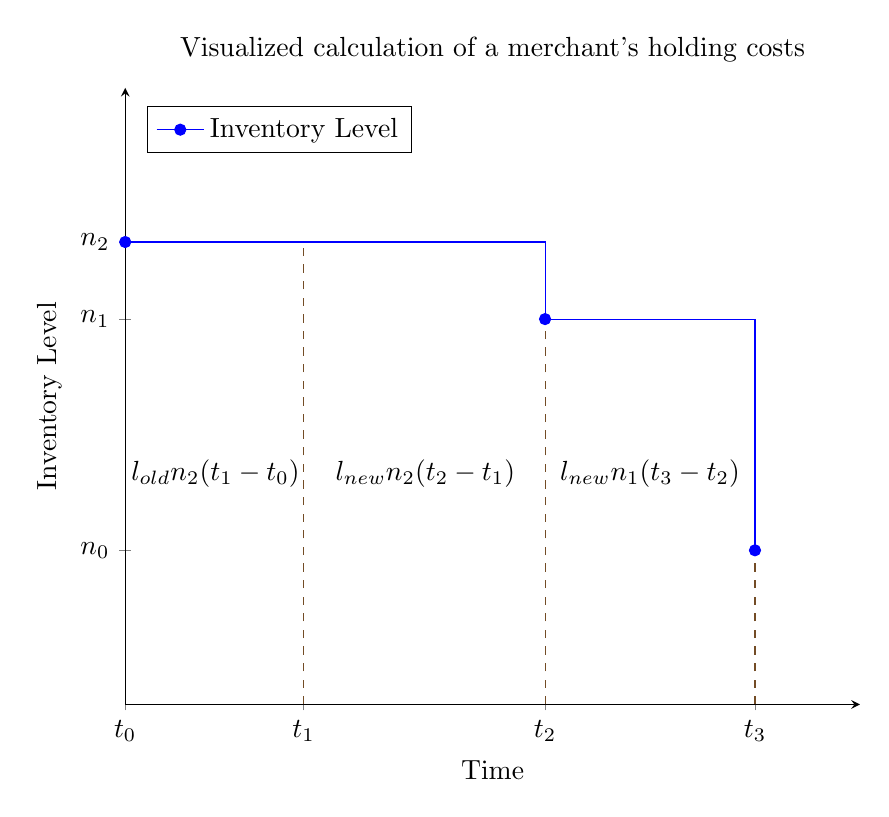
\begin{tikzpicture}
\begin{axis}[
title={Visualized calculation of a merchant's holding costs},
xlabel={Time},
ylabel={Inventory Level},
xmin=0, xmax=3.5,
ymin=0, ymax=8,
xtick={0,0.85,2,3},
xticklabels={$t_0$,$t_1$,$t_2$,$t_3$},
ytick={2,5,6},
yticklabels={$n_0$,$n_1$,$n_2$},
legend pos=north west,
grid style=dashed,
axis lines = left,
width=0.9\textwidth,
]

\addplot[color=blue,mark=*,const plot mark left]
coordinates {(0,6)(2,5)(3,2)};
\legend{Inventory Level}

\addplot[color=brown!60!black,dashed]
coordinates {(0.85,0)(0.85,6)};

\addplot[color=brown!60!black,dashed]
coordinates {(2,0)(2,5)};

\addplot[color=brown!60!black,dashed]
coordinates {(3,0)(3,2)};

\node[] at (axis cs: 0.43,3) {$l_{old} n_2 (t_1 - t_0) $};
\node[] at (axis cs: 1.43,3) {$l_{new} n_2 (t_2 - t_1) $};
\node[] at (axis cs: 2.5,3) {$l_{new} n_1 (t_3 - t_2) $};

\end{axis}
\end{tikzpicture}
%area under graph
\caption[Holding costs calculation]{Whenever a merchant's inventory level or holding cost rate changes, the holding costs since the previous change are computed.
	Holding costs depend on the holding cost rate, the inventory level, and time since the last change.
	Holding costs are proportional to the area under the graph segment.
	At $t_1$ the holding cost rate changes from $l_{old}$ to $l_{new}$.}
\label{fig:holding_cost}
\end{figure}

%write about connected streams?
The computation of holding costs is triggered every time a merchant's inventory level or holding cost rate changes.
In that case, the holding costs since the last change are calculated.
\cref{fig:holding_cost} shows an example of this process.
%check: formulate this as equation
The holding costs of the interval between two consecutive events is the inventory level multiplied with the duration and the holding cost rate.
Note that changes in inventory level or holding cost rate can happen at any time and are not periodically.
%motivate why this implementation; what is alternative (calc periodically)?

\section{Delivery Time}
\label{section:shipping_time}
%what
After a merchant orders items from the producer, some time should pass until the items arrive at the merchant.
This is the delivery time from producer to merchant.
Previously on the \pricewars platform, merchants received ordered products instantly.
%why
Merchants must think ahead of time while ordering to receive the products at the right time.
If merchants underestimate demand, they risk stock-outs before the ordered products arrive.
The addition of delivery time will result in a more realistic competition between merchants on the online marketplace.

%how
Previously, merchants made a HTTP request to the producer for an order and the response contained the ordered items.
To add a delivery time to this process, we considered three approaches: long-running HTTP requests, web sockets, and two separate HTTP requests. 

Long-running HTTP requests are the simplest solution to implement delivery time.
The producer creates the ordered items and waits a certain time to respond.
However, this approach is problematic due to timeouts and may block execution of the producer or merchant.
We decided against long-running requests.

Web sockets are a flexible alternative to HTTP requests and create a bi-directional connection.
The merchant opens a web socket to the producer, then sends an order over the web socket.
The producer can send the ordered items at any time as a response.
When the merchant received the items, the web socket can be closed or kept open for additional orders.
The consensus on the usage of web sockets is that they should not be used to replicate request-response communication.
Thus web sockets are not the optimal solution to implement delivery time and we used the third approach, two separate requests.

The process of ordering and receiving products is split into two separate HTTP requests.
The merchant creates a new order with an order request.
The producer responds with an estimated time until the order is ready.
If the delivery time is over, the merchant can make a request to receive the ordered items from the producer.
The producer only returns the ordered items if the delivery time is over.
An order can only be received once.

This solution requires an additional HTTP request compared to instant orders.
This is only a small additional overhead and it is easy to update existing merchants to the new ordering process.
but this is only a small overhead and uses common web technologies.
The known duration until the order is ready is advantageous for this approach.
The merchant does not need to poll the producer until the order is ready.

\section{Inventory Visualization}
\label{section:inventory_graph}

\begin{figure}[t]
	\centering
	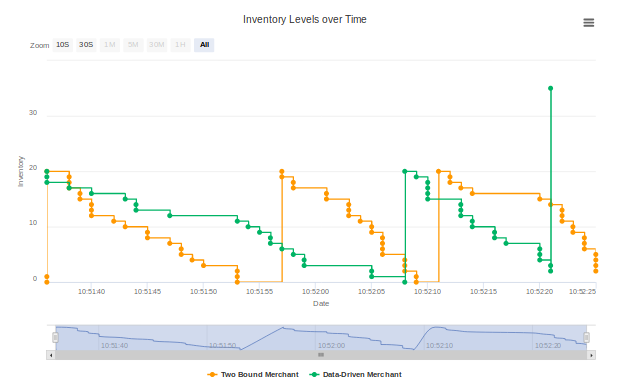
\includegraphics[width=0.8\textwidth]{figures/inventory_graph}
	\caption{Chart from the management UI showing the inventory levels over time of two competing merchants.}
	\label{fig:invnetory_graph}
\end{figure}

%more motivation?
The platform extensions create the inventory control problem for merchants.
Merchants' inventory levels are more important than ever before because of this problem.
In order to analyze how merchants control their inventory levels, we added an inventory chart to the management UI.
Users have access to the new chart that shows inventory levels over time from all merchants.
\cref{fig:invnetory_graph} shows an example of the inventory chart.
This chart is shown along other charts, which present metrics like prices, profit, and revenue. 
We used the highcharts\footnote{Javascript chart library, Highcharts: \url{https://www.highcharts.com/}} library to have the same look and feel as the existing charts.

\section{Benchmarking Tool}
\label{section:benchmark_tool}
%problem
Getting comparable results over multiple simulations on the \pricewars platform was problematic while developing our merchant.
The charts on the management UI are great to evaluate a single simulation run but it is not precise enough to compare multiple runs.
It is not feasible to manually examine charts at an exact timing.
A better way to compare simulation runs with each other is especially important in monopoly scenarios, when merchant with different configurations or strategies are compared.

%solution
%check: need to explain events?
We developed a benchmarking tool that runs the \pricewars platform for a certain duration with specified merchants.
This tool allows the user to run simulations the same duration and they do not have to read a chart at the right point in time.
After a run, the benchmark tool saves all events from the event log.
Events are analyzed to determine each merchant's profit, revenue, and expenses as shown in \cref{tab:benchmark_tool}.
Users can run additional analysis afterwards on the saved events, e.g. how many stock-outs had each merchant.
Another benefit from using the benchmark tool is the automated setup and teardown of the platform.
This process would need some manual steps otherwise.

\begin{table}[t]
\centering
\begin{tabular}{ lrrrr }
	\toprule
	Merchant & Profit & Revenue & Holding Cost & Order Cost \\
	\midrule
	Merchant A & 534.17 & 3\,547.00 & 212.83 & 2\,800.00 \\
	Merchant B & 315.12 & 4\,063.80 & 363.80 & 3\,385.00 \\
	Merchant C & 492.50 & 3\,844.80 & 152.30 & 3\,200.00 \\
	\bottomrule
\end{tabular}
\caption{The benchmark tool generates a breakdown of expenses and revenues. These are results from a five minute simulation.}
\label{tab:benchmark_tool}
\end{table}

%todo implemenation? calls docker-compose, start merchants directly
	
\chapter{Conclusion}
%plus future work

%mention applications for my solution

%until now only comparison to rule-base merchants
%basis/comparison for new merchants

%data-driven outperforms rule-based if enough datat collected
	%%!TEX root = ../thesis.tex
	\clearpage
%	\printglossary[type=\acronymtype,style=modsuper]
	\bibliography{sources.bib}
%	\begin{appendices}
%	%!TEX root = ../thesis.tex
\chapter{Notation Table}

%\begin{table}[t]
%	\centering
%	\begin{tabular}{ ll }
\begin{longtable}{ll}
		\toprule
		\textbf{Symbol} & \textbf{Description} \\
		\midrule
		$a_{fix}$ & Fixed selling price. \\
		$\delta$ & Discount factor for future profits. \\
		$l$ & Holding costs per item and period. \\
		$t$ & Identifier variable for a time period. \\
		$N_t$ & Random inventory level at the start of period $t$. \\
		$b_t$ & Number of items ordered at start of period $t$. \\
		$B$ & Set of admissible order quantities. \\
		$c_{fix}$ & Fixed order costs. \\
		$c_{var}$ & Variable order costs. \\
		$C(b)$ & Total order costs for ordering $b$ items. \\
		$P(i)$ & Probability to sell i items in one time period. \\
		% P(i,a)
		$X_t$ & Random number of sold items in period $(t-1, t)$. \\
		$G_t$ & Random accumulated discounted profit from period $t$. \\
		$n$ & Inventory level. \\
		$V_t(n)$ & \makecell[l]{Value function: best expected discounted profit from \\ period $t$ with a start inventory of $n$ items.} \\
		$T$ & Number of periods of the limited time horizon. \\
		$N_{max}$ & Maximum inventory capacity. \\
		$b$ & Order quantity. \\
		$u$ & Start value for value function: $V_T(n) = u, 0 \leq n \leq N_{max}$. \\
		$b^*(n)$ & \makecell[l]{Optimal ordering decision with delayed orders \\ for inventory level of $n$.} \\
		$b^*_{instant}(n)$ & Same as $b^*(n)$ but for instantaneous orders. \\
		$A$ & Set of admissible pricing decision. \\
		$a_t$ & Offer price at time $t$. \\
		$a^*(n)$ & Optimal pricing decision for inventory level of $n$. \\
		$\vec{s}$ & Market situation, vector of merchant offers. \\
		%todo change to x(a, s)
		$\vec{x}(\vec{s})$ & Explanatory variables for market situation $\vec{s}$. \\
		$\lambda(\vec{s}; \vec{\beta})$ & Estimated mean sales in one period. \\
		$\vec{\beta}$ & Weights vector for linear regression. \\
		$\vec{\beta}^*$ & Optimal weights for specific trainings data. \\
		$\gamma(a)$ & \makecell[l]{Probability for a single customer of buying an item. \\ Used for binomial distribution.} \\
		$V_0^{old}(n)$ & Result of value function from last computation. \\
		\bottomrule
%	\end{tabular}
	\caption[List of Variables and Parameters]{List of variables and parameters with description.}
	\label{tab:notations}
%\end{table}
\end{longtable}

%	\end{appendices}
	%!TEX root = thesis.tex
%\selectlanguage{german}
\chapter*{Eigenst"andigkeitserkl"arung}
Ich erkl"are hiermit, dass ich die vorliegende Arbeit selbst"andig verfasst und keine anderen als die genannten Quellen und Hilfsmittel verwendet habe.
\\
\\
\\
\\
\\
Potsdam, \today
\\
\\
\\
\\
\AUTHOR

\end{document}
